\section{Key-value database}

Key-value databases store data as a collection of key-value pairs, where each key acts as a unique identifier that points to a corresponding value. 
This structure allows for efficient retrieval of data, making key-value databases particularly useful in scenarios that require fast lookups by key. 
Conceptually, the key-value approach is analogous to indexing in relational databases, where a key serves as a reference to access the associated data object.

Key-value databases are often used as the foundation for applications requiring high performance in terms of speed and scalability, and they form the backbone for search operations by id.

\subsection{Redis}
Key features of Redis include:
\begin{itemize} 
    \item \textit{Advanced data structures}: Redis values can be more than just simple strings or numbers—they can represent data structures like lists, sets, or even geospatial indexes. 
    \item \textit{Atomic operations}: Redis supports atomic operations on its native data structures, ensuring that operations on a specific data type can be completed without interference from other operations. 
    \item \textit{Versatility}: Redis can be used as a persistent database, a fast in-memory cache, or a message broker, making it a multi-purpose tool in modern architectures. 
\end{itemize}
Redis follows a unique path in the evolution of key-value databases, as it directly exposes complex data types as part of its interface, without adding extra abstraction layers. 
This makes Redis particularly well-suited for use cases where performance and simplicity are critical.

While Redis is not a direct replacement for relational databases or document stores, it complements them well. 
Redis can be used alongside SQL databases for fast access to frequently queried data, or alongside NoSQL databases to provide rapid access to specific data sets.

Best use cases for Redis are: 
\begin{itemize} 
    \item When speed is crucial and you need real-time data processing. 
    \item When you need more than basic key-value pairs, and complex data structures are required. 
    \item When the dataset can fit into memory, allowing for in-memory storage to maximize performance.
     \item When the dataset is non-critical, as Redis persistence mechanisms can add latency, which might not be ideal for mission-critical applications. 
\end{itemize}

\paragraph*{Architecture}
Redis was written in ANSI C by Salvatore Sanfilippo. 
It is designed to run on most POSIX-compliant systems like Linux, BSD, and macOS, with Linux being the recommended platform for production use.

While Redis is a single-threaded server, it can scale across multiple CPU cores by running several Redis instances in parallel. 
Redis guarantees that all operations are atomic, meaning no two commands will be executed concurrently.
Many Redis commands are executed with constant time complexity, making them highly efficient even at scale. 

Redis does not natively support Windows, but Microsoft maintains an open-source 64-bit Windows port of Redis.
\begin{figure}[H]
    \centering
    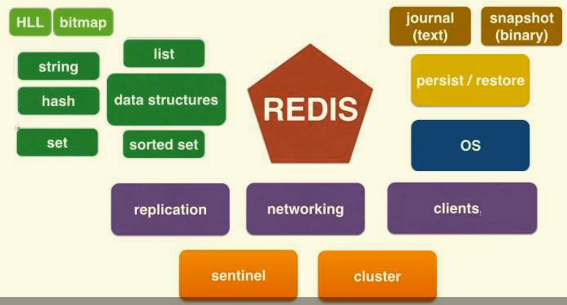
\includegraphics[width=0.75\linewidth]{images/redis.png}
    \caption{Redis architecture}
\end{figure}
